
\begin{comment}
\begin{frame}{Continuous Query Engine: $\mathsf{DP_{ATM}}$}
    \begin{figure}
        \hspace*{-1cm} % adjust the value to control the leftward shift
        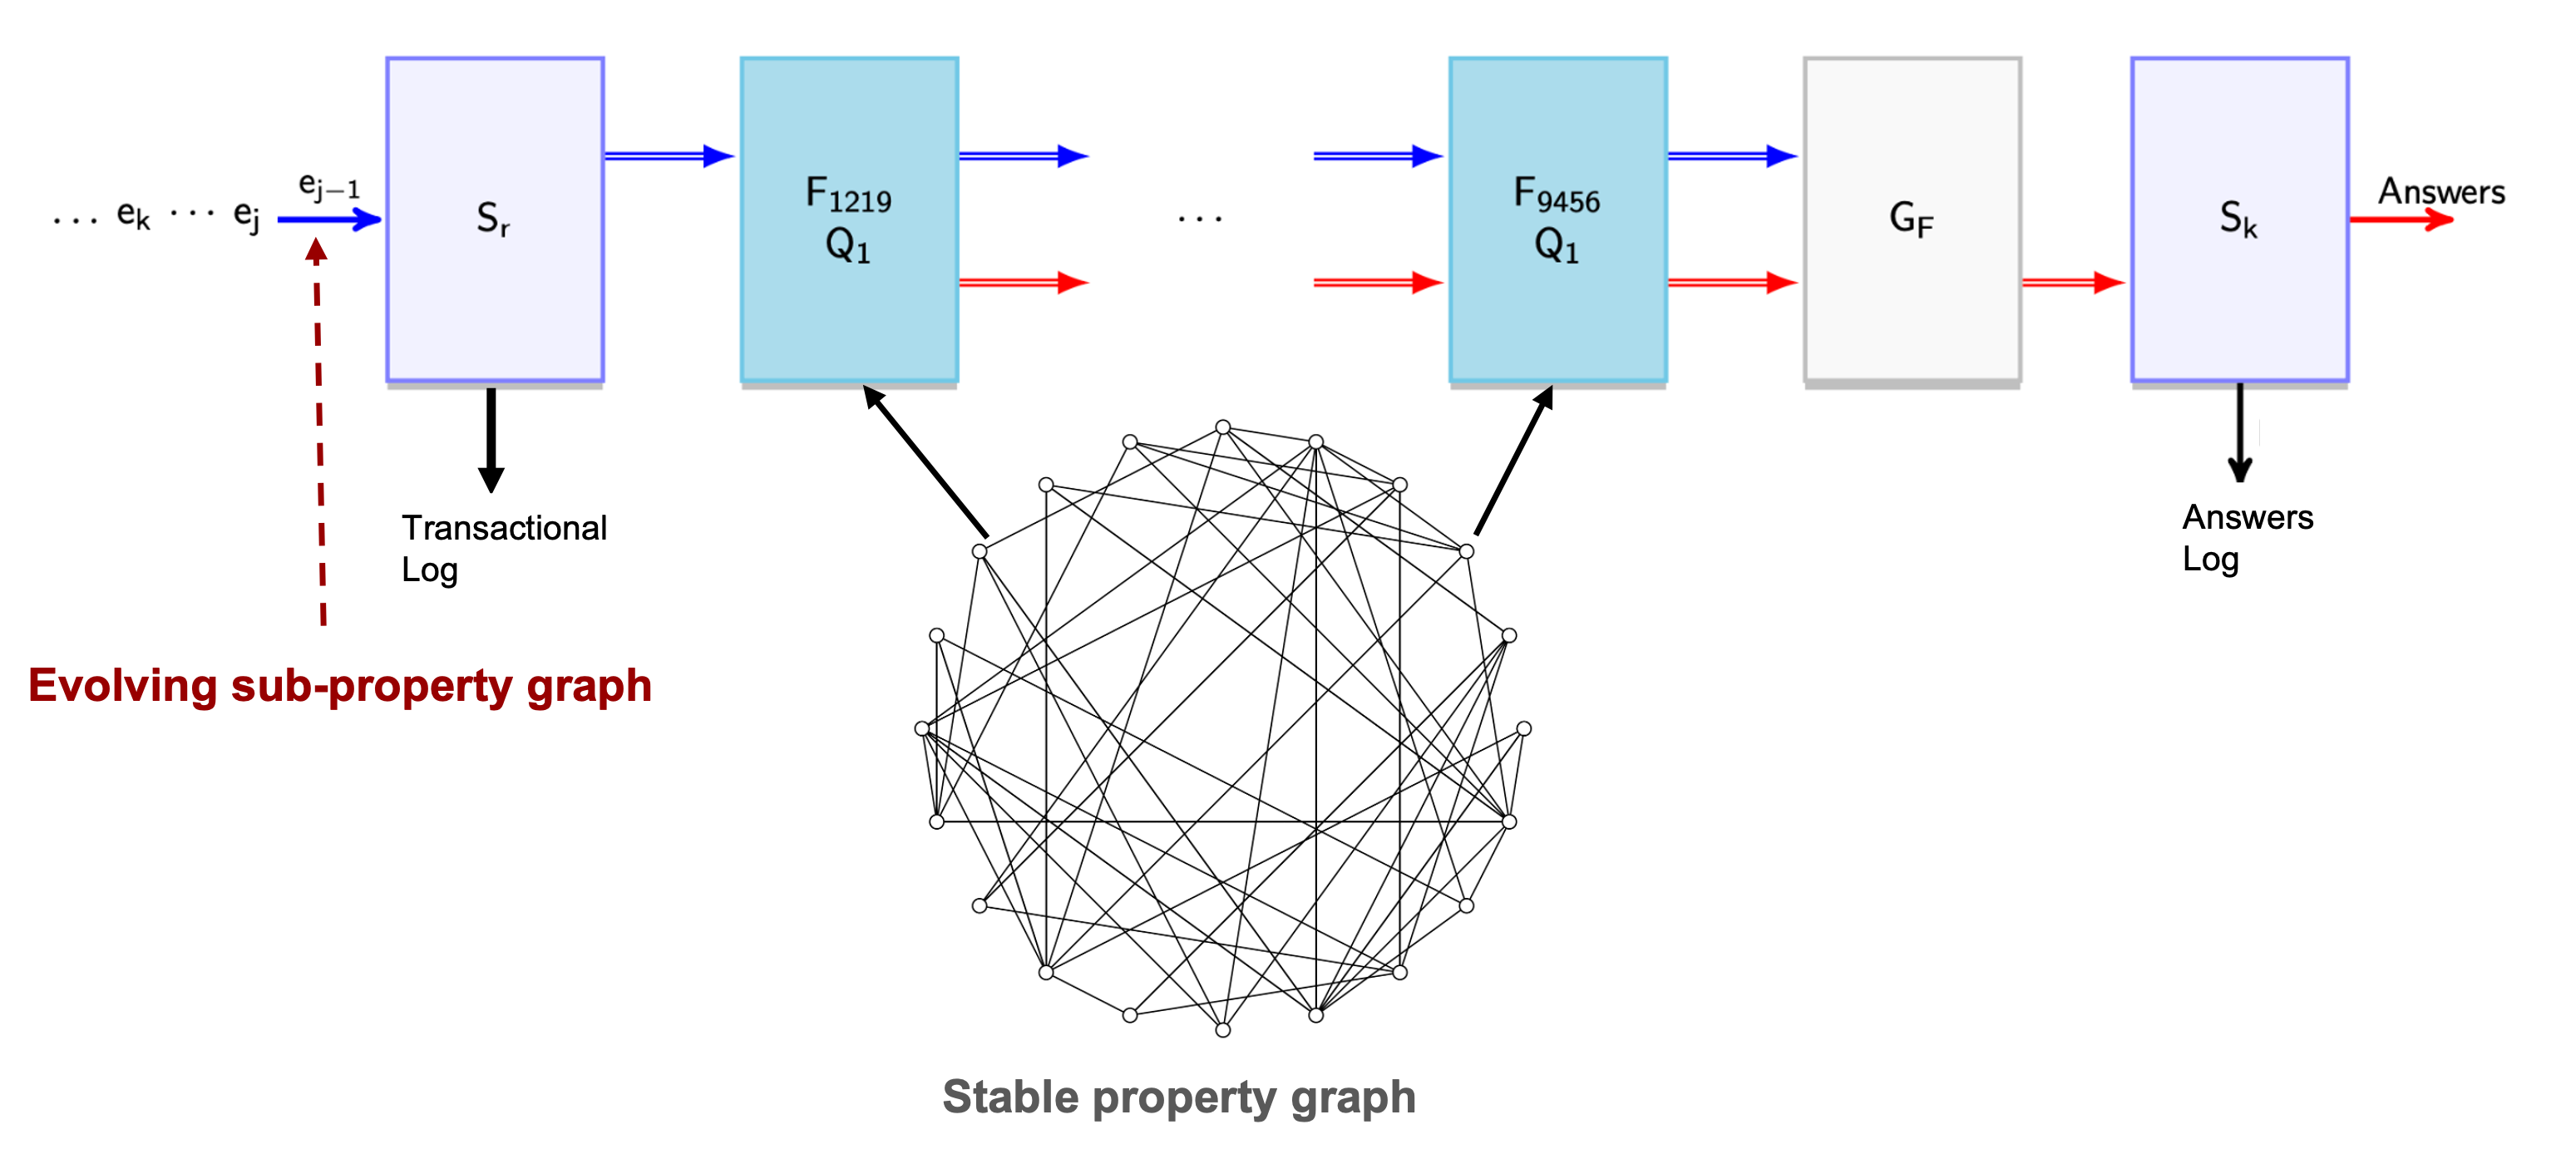
\includegraphics[width=1.2\textwidth]{figures/architecture.png}
    \end{figure}
\end{frame}
\end{comment}

\begin{comment}
\begin{frame}{$\mathsf{DP_{ATM}}$ - Input Stream}
\textbf{Note}: 2 edges per transaction - the \emph{opening} edge and the \emph{closing} edge.

\begin{figure}
    \centering
    \only<1>{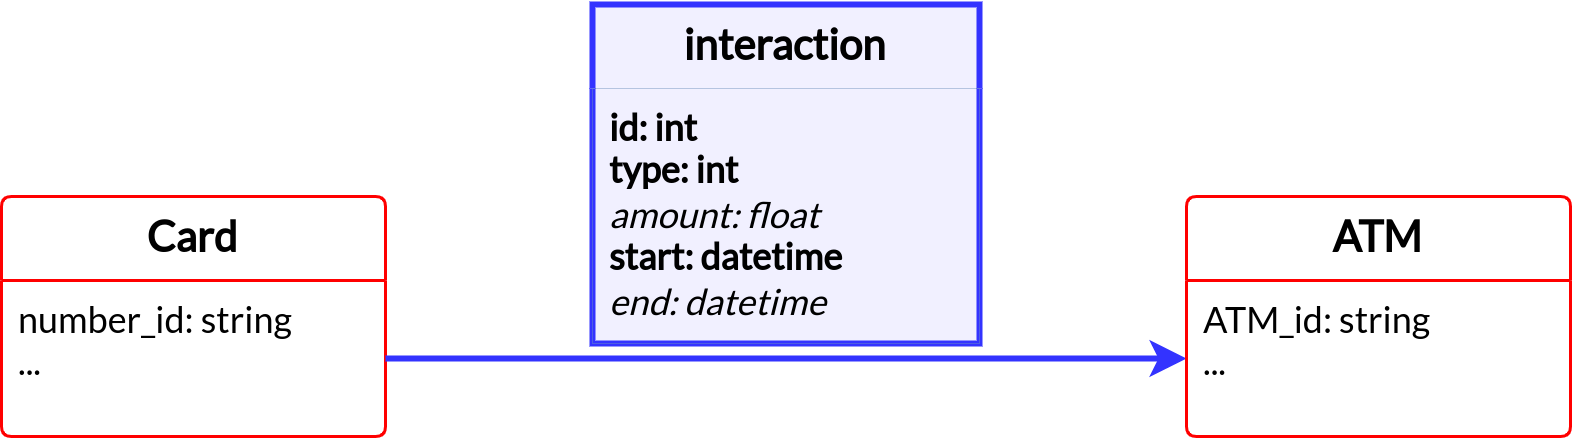
\includegraphics[width=\textwidth]{images/1-DataModel/2-edges-tx-tfm.png}}
    \only<2>{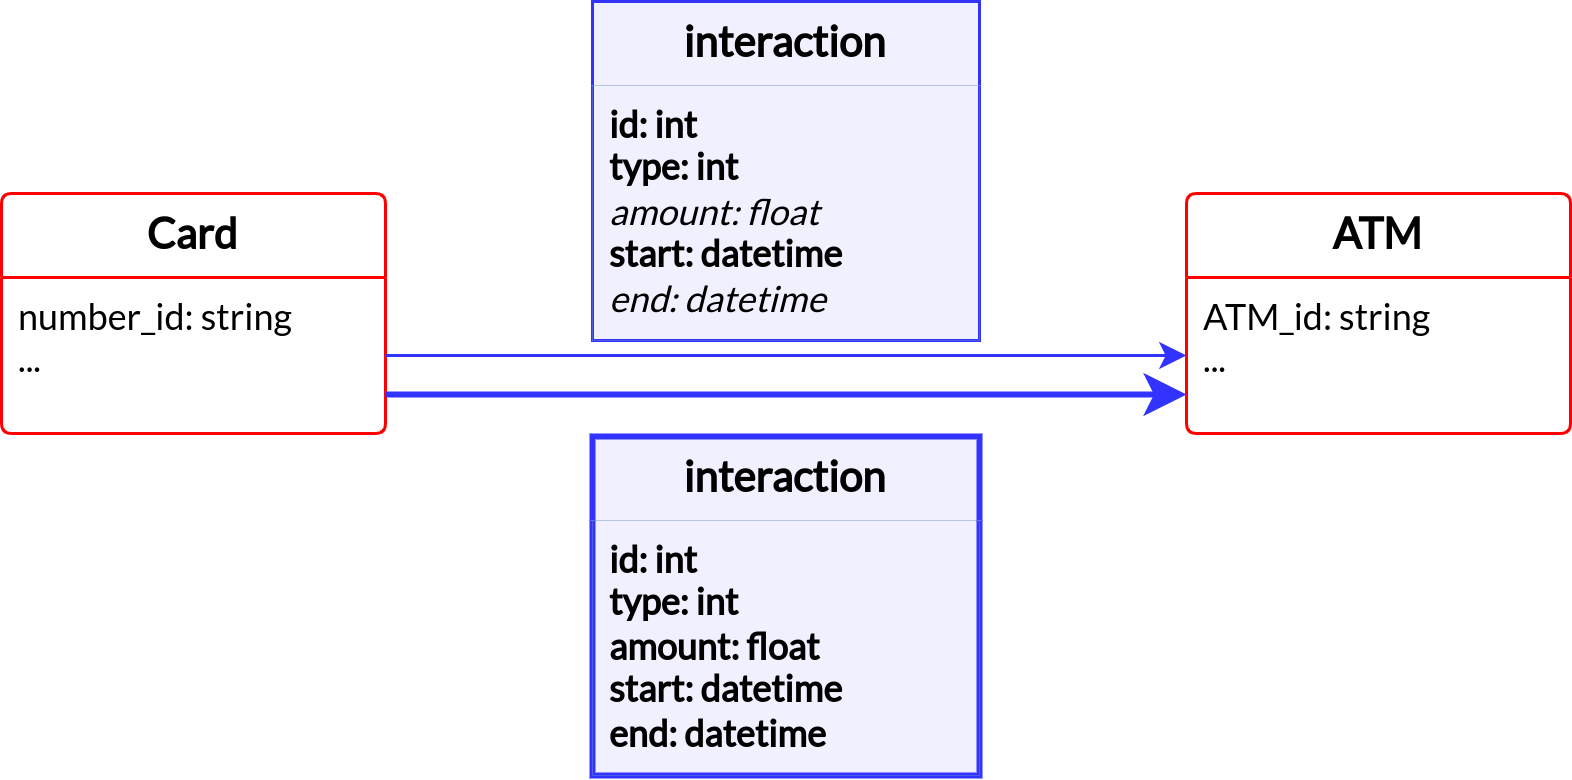
\includegraphics[width=\textwidth]{images/1-DataModel/2-edges-tx-tfm-1.png}}
    \caption{\only<1>{Opening edge}\only<2>{Closing edge}}
\end{figure}
\end{frame}
\end{comment}

\begin{frame}{Continuous Query Engine - $\mathsf{DP_{ATM}}$: Stages}
    \begin{itemize}
        \item<1-> \textbf{Source:} Manages the in-connection with the outside: streaming input / file reading... \& general transactions log.
        \item<2-> \textbf{Sink:} Manages the out-connection. Outside answers/alerts emission \& alert log.
        \item<3-> \textbf{Generator:} Generation of new filters.
        \item<4-> \textbf{Filter:} (Stateful) stage. Anomalous detection tracking process of \emph{maxFilterSize} cards.
    \end{itemize}
    \begin{figure}
    \hspace*{-0.9cm}
    \centering
    \only<1>{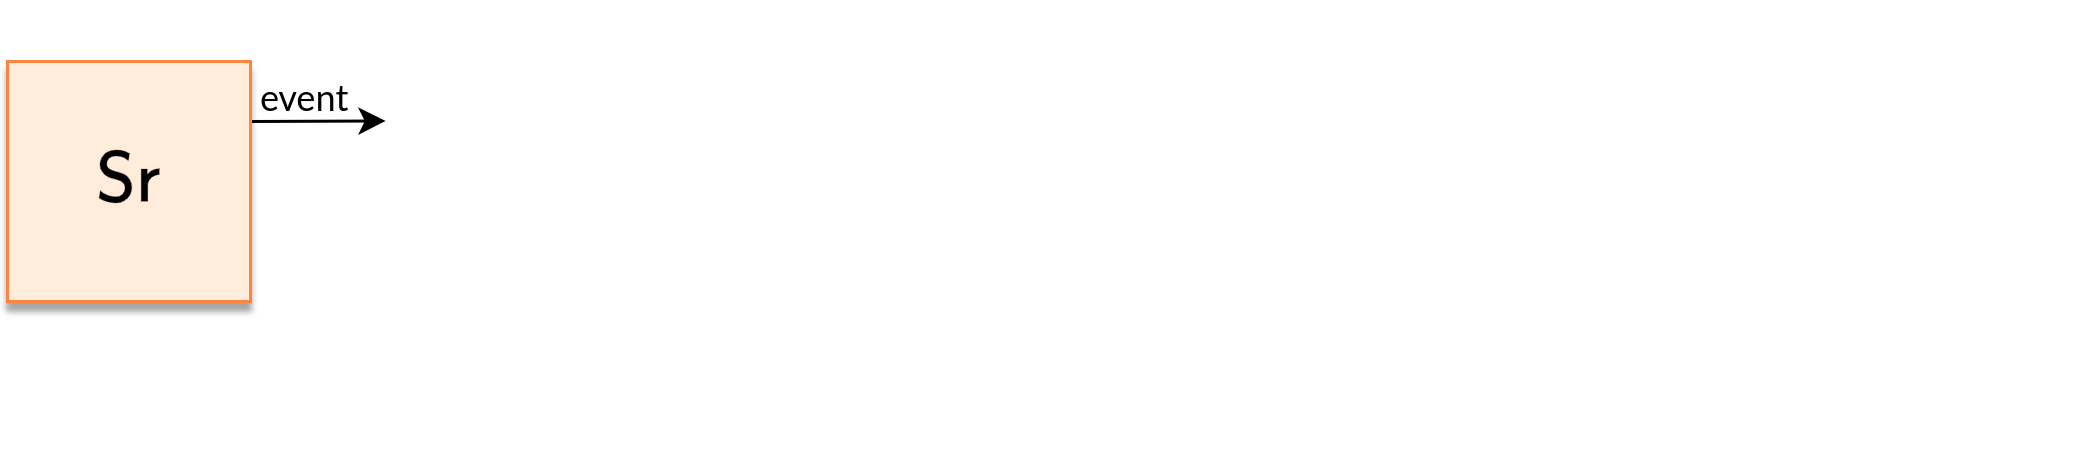
\includegraphics[scale=0.7]{images/Source.png}}
    \only<2>{\hspace{-0.1cm}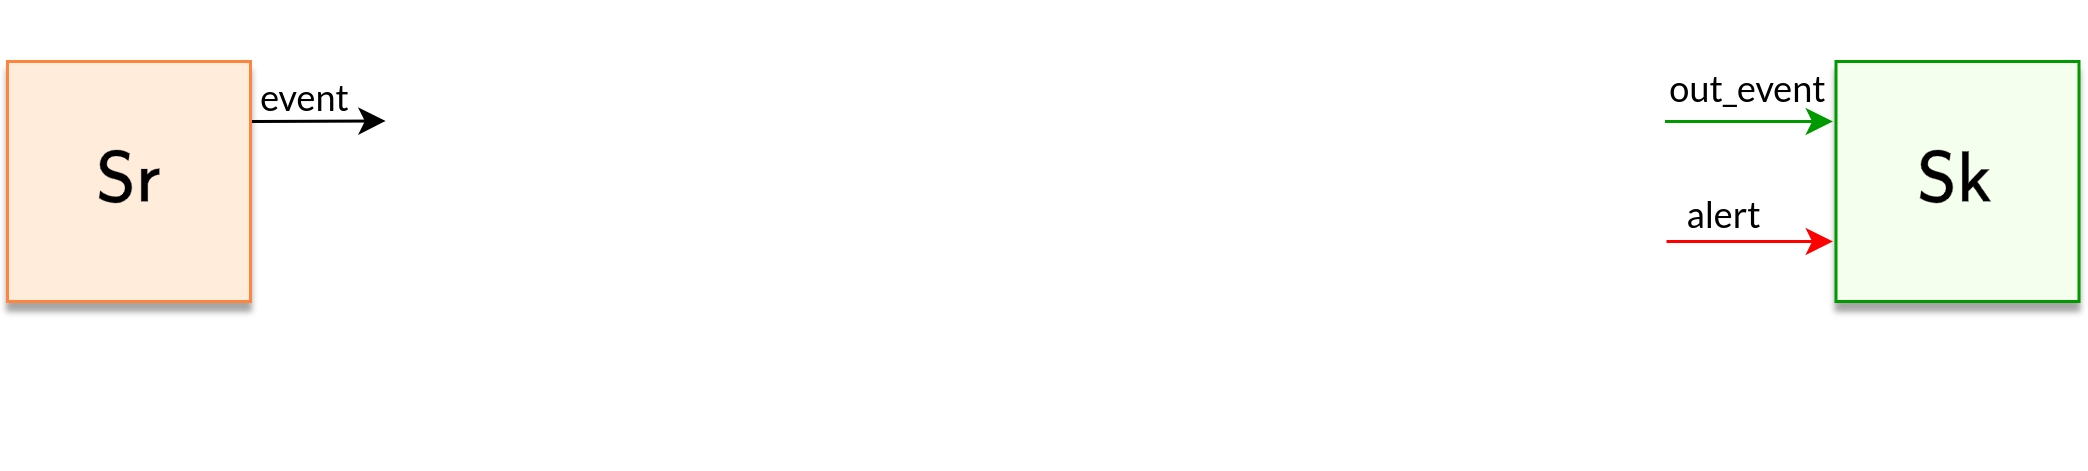
\includegraphics[scale=0.7]{images/Sink.png}}
    \only<3>{\hspace{-0.1cm}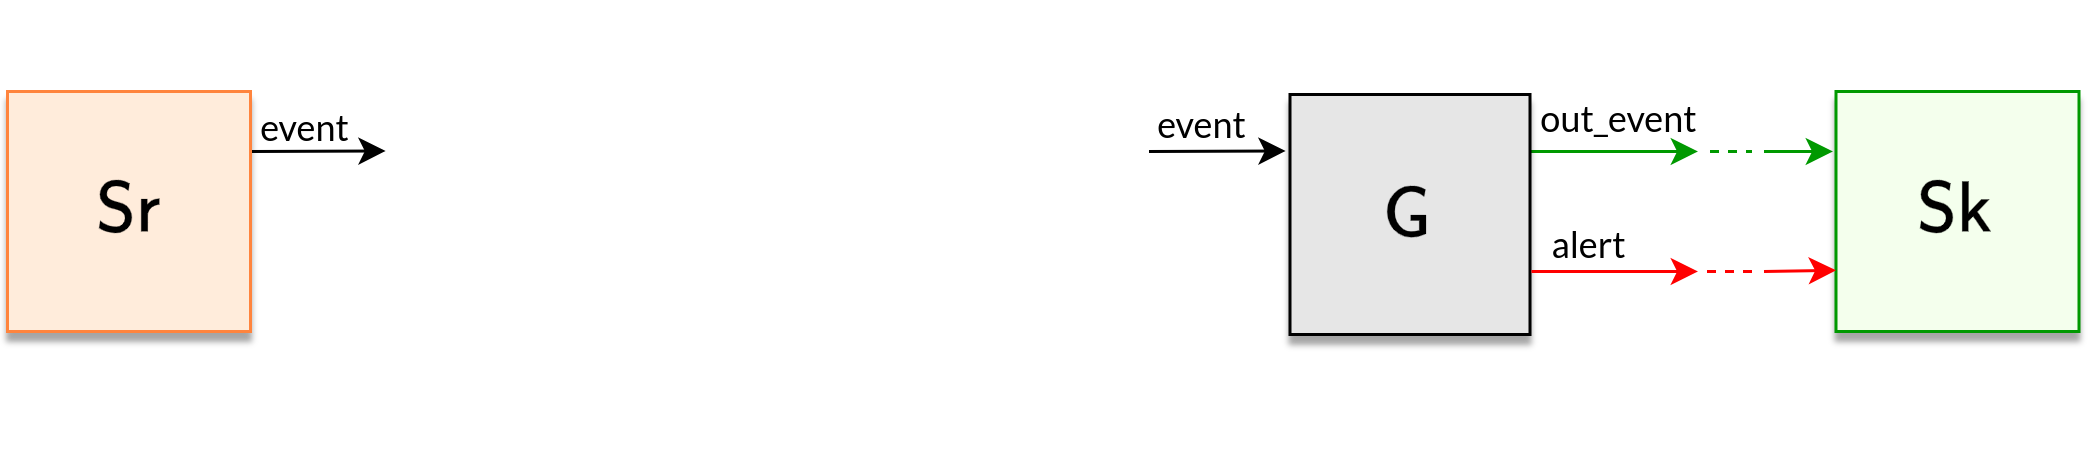
\includegraphics[scale=0.7]{images/Generator.png}}
    \only<4>{\hspace{-0.2cm}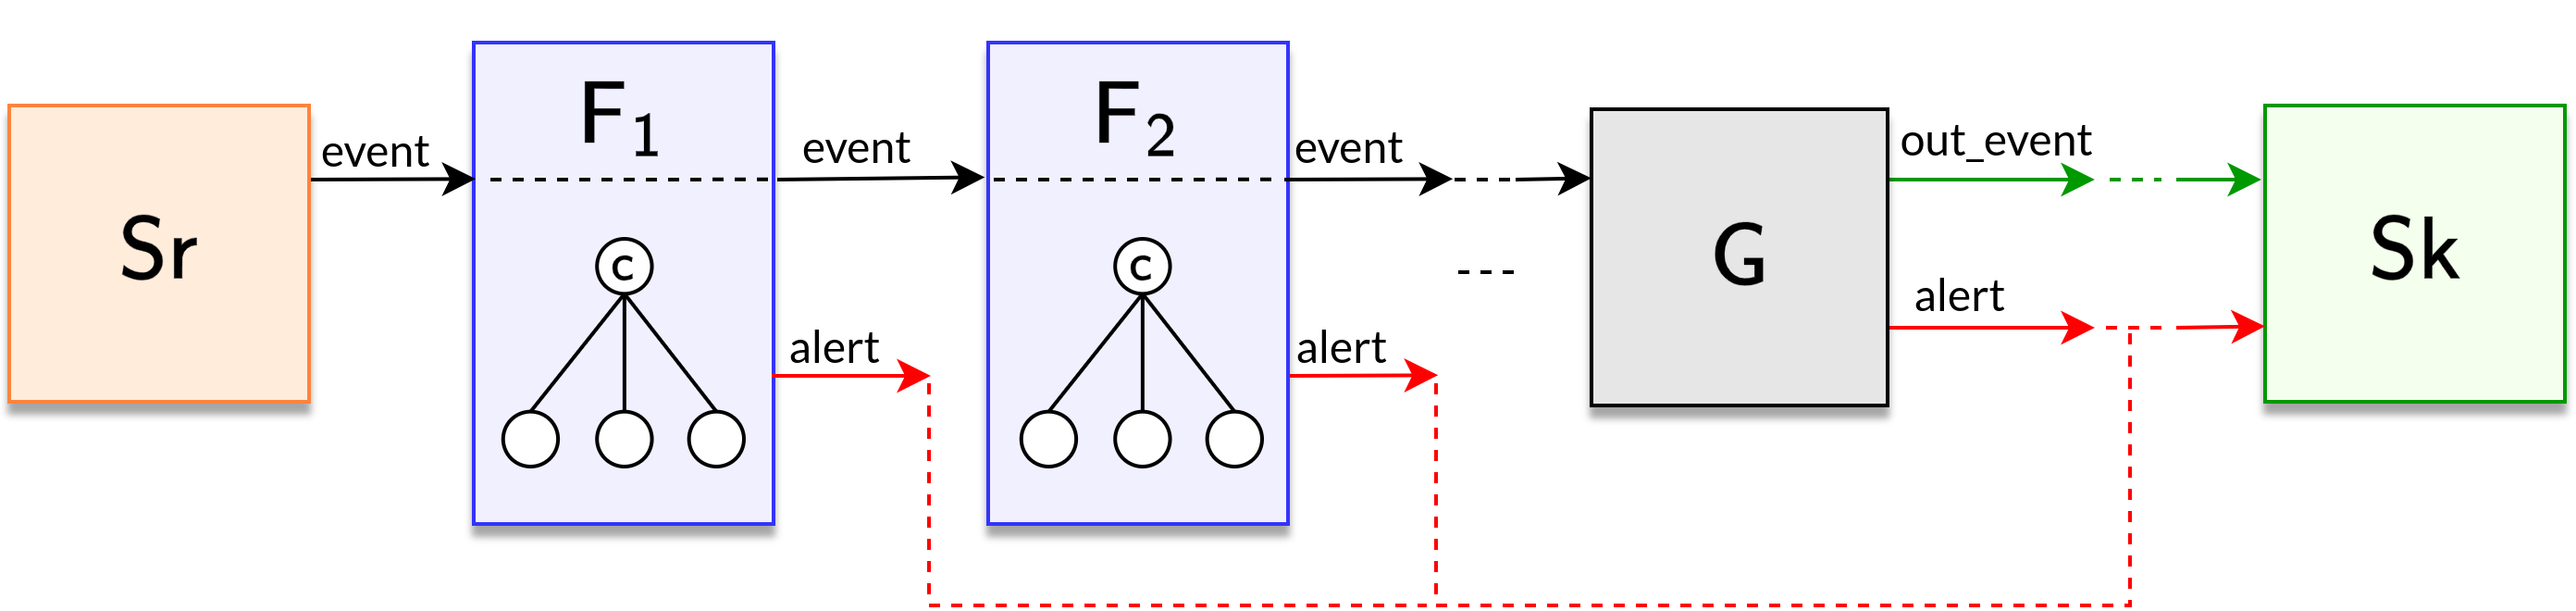
\includegraphics[scale=0.7]{figures/Filter-edit.png}}
\end{figure}
\end{frame}


\begin{comment}
\begin{frame}{$\mathsf{DP_{ATM}}$ - Stages}
    \begin{itemize}
        \item<1-> \textbf{Source:} Manages the in-connection with the outside: streaming input / file reading... \& general transactions log.
        \item<2-> \textbf{Sink:} Manages the out-connection. Outside answers/alerts emission \& alert log.
        \item<3-> \textbf{Generator:} Generation of new filters.
        \item<4-> \textbf{Filter:} (Stateful) stage. Anomalous detection tracking process of \emph{maxFilterSize} cards.
    \end{itemize}
    
    \centering
    \vspace{-0.5cm}
    \begin{adjustwidth}{-0.7cm}{}
    \begin{tikzpicture}
        \begin{pgfonlayer}{nodelayer}
            \node [style=io, minimum height=1.25cm, minimum width=3.5cm, shape border rotate=270, visible on=<1->] (0) at (-4.5, 0) {Source};
            \node [style=filter_gen, minimum width=1cm, minimum height=2.5cm, visible on=<4->] (1) at (-2, 0) {Filter};
            \node [style=filter_gen, minimum width=1cm, minimum height=2.5cm, visible on=<4->] (2) at (0.4, 0) {Filter};
            \node [style=filter_gen, minimum width=1cm, minimum height=2.5cm, align=center, visible on=<3->] (3) at (3, 0) {Generator \\ 
\includegraphics[width=.05\textwidth]{gear} };
            \node [style=io, minimum height=1.25cm, minimum width=3.5cm, shape border rotate=90, visible on=<2->] (4) at (5.7, 0) {Sink};
        \end{pgfonlayer}
        \begin{pgfonlayer}{edgelayer}
            \draw [style={opChan}, visible on=<5->] ([yshift=0.5 cm]0.east) to["$e_i$"] ([yshift=0.5 cm]1.west);
            \draw [style={opChan}, visible on=<5->] ([yshift=0.5 cm]1.east) to["$e_i$"] ([yshift=0.5 cm]2.west);
            \draw [style={opChan}, visible on=<5->] ([yshift=0.5 cm]2.east) to["$e_i$"] ([yshift=0.5 cm]3.west);
            
            \draw [style={daChan}, visible on=<5->] ([yshift=-0.5 cm]1.east) to["Alerts"] ([yshift=-0.5 cm]2.west);
            \draw [style={daChan, visible on=<5->}] ([yshift=-0.5 cm]2.east) to["Alerts"] ([yshift=-0.5 cm]3.west);
            \draw [style={daChan}, visible on=<5->] ([yshift=-0.5 cm]3.east) to["Alerts"] ([yshift=-0.5 cm]4.west);
        \end{pgfonlayer}
        \node (down0) at (-4.5, -2.55);
        \draw [[-{Stealth[length=4mm]}, alt=<1>{red}{black}] (0) to["log"] (down0);
        
        \node (down4) at (5.7, -2.55);
        \draw [[-{Stealth[length=4mm]}, visible on=<2->, alt=<2>{red}{black}] (4) to["log" '] (down4);
        
        \node (right4) at (7.4, 0);
        \draw [[-{Stealth[length=4mm]}, visible on=<2->, red] (4) to["Alerts"] (right4);
    \end{tikzpicture}
    \end{adjustwidth}
\end{frame}
\end{comment}

\begin{frame}{Continuous Query Engine - $\mathsf{DP_{ATM}}$: Filter Stage}
    \begin{columns} % Create two columns
        % Left column for the item list
        \begin{column}{0.5\textwidth}
            \begin{itemize}
                \item Stores the \textbf{induced card subgraph(s)} of the incoming belonging edges.
                \item Evaluation of continuous query pattern(s). Each has a \textbf{connection} session with the \textbf{stable gdb}.
                \item Emission of \textbf{alerts} in case of matching a query pattern.
                \item Filter \emph{worker} $\mathsf{FW}$ to avoid bottlenecks - \emph{in parallel}.
            \end{itemize}
        \end{column}

        % Right column for the image
        \begin{column}{0.6\textwidth}
            \centering
            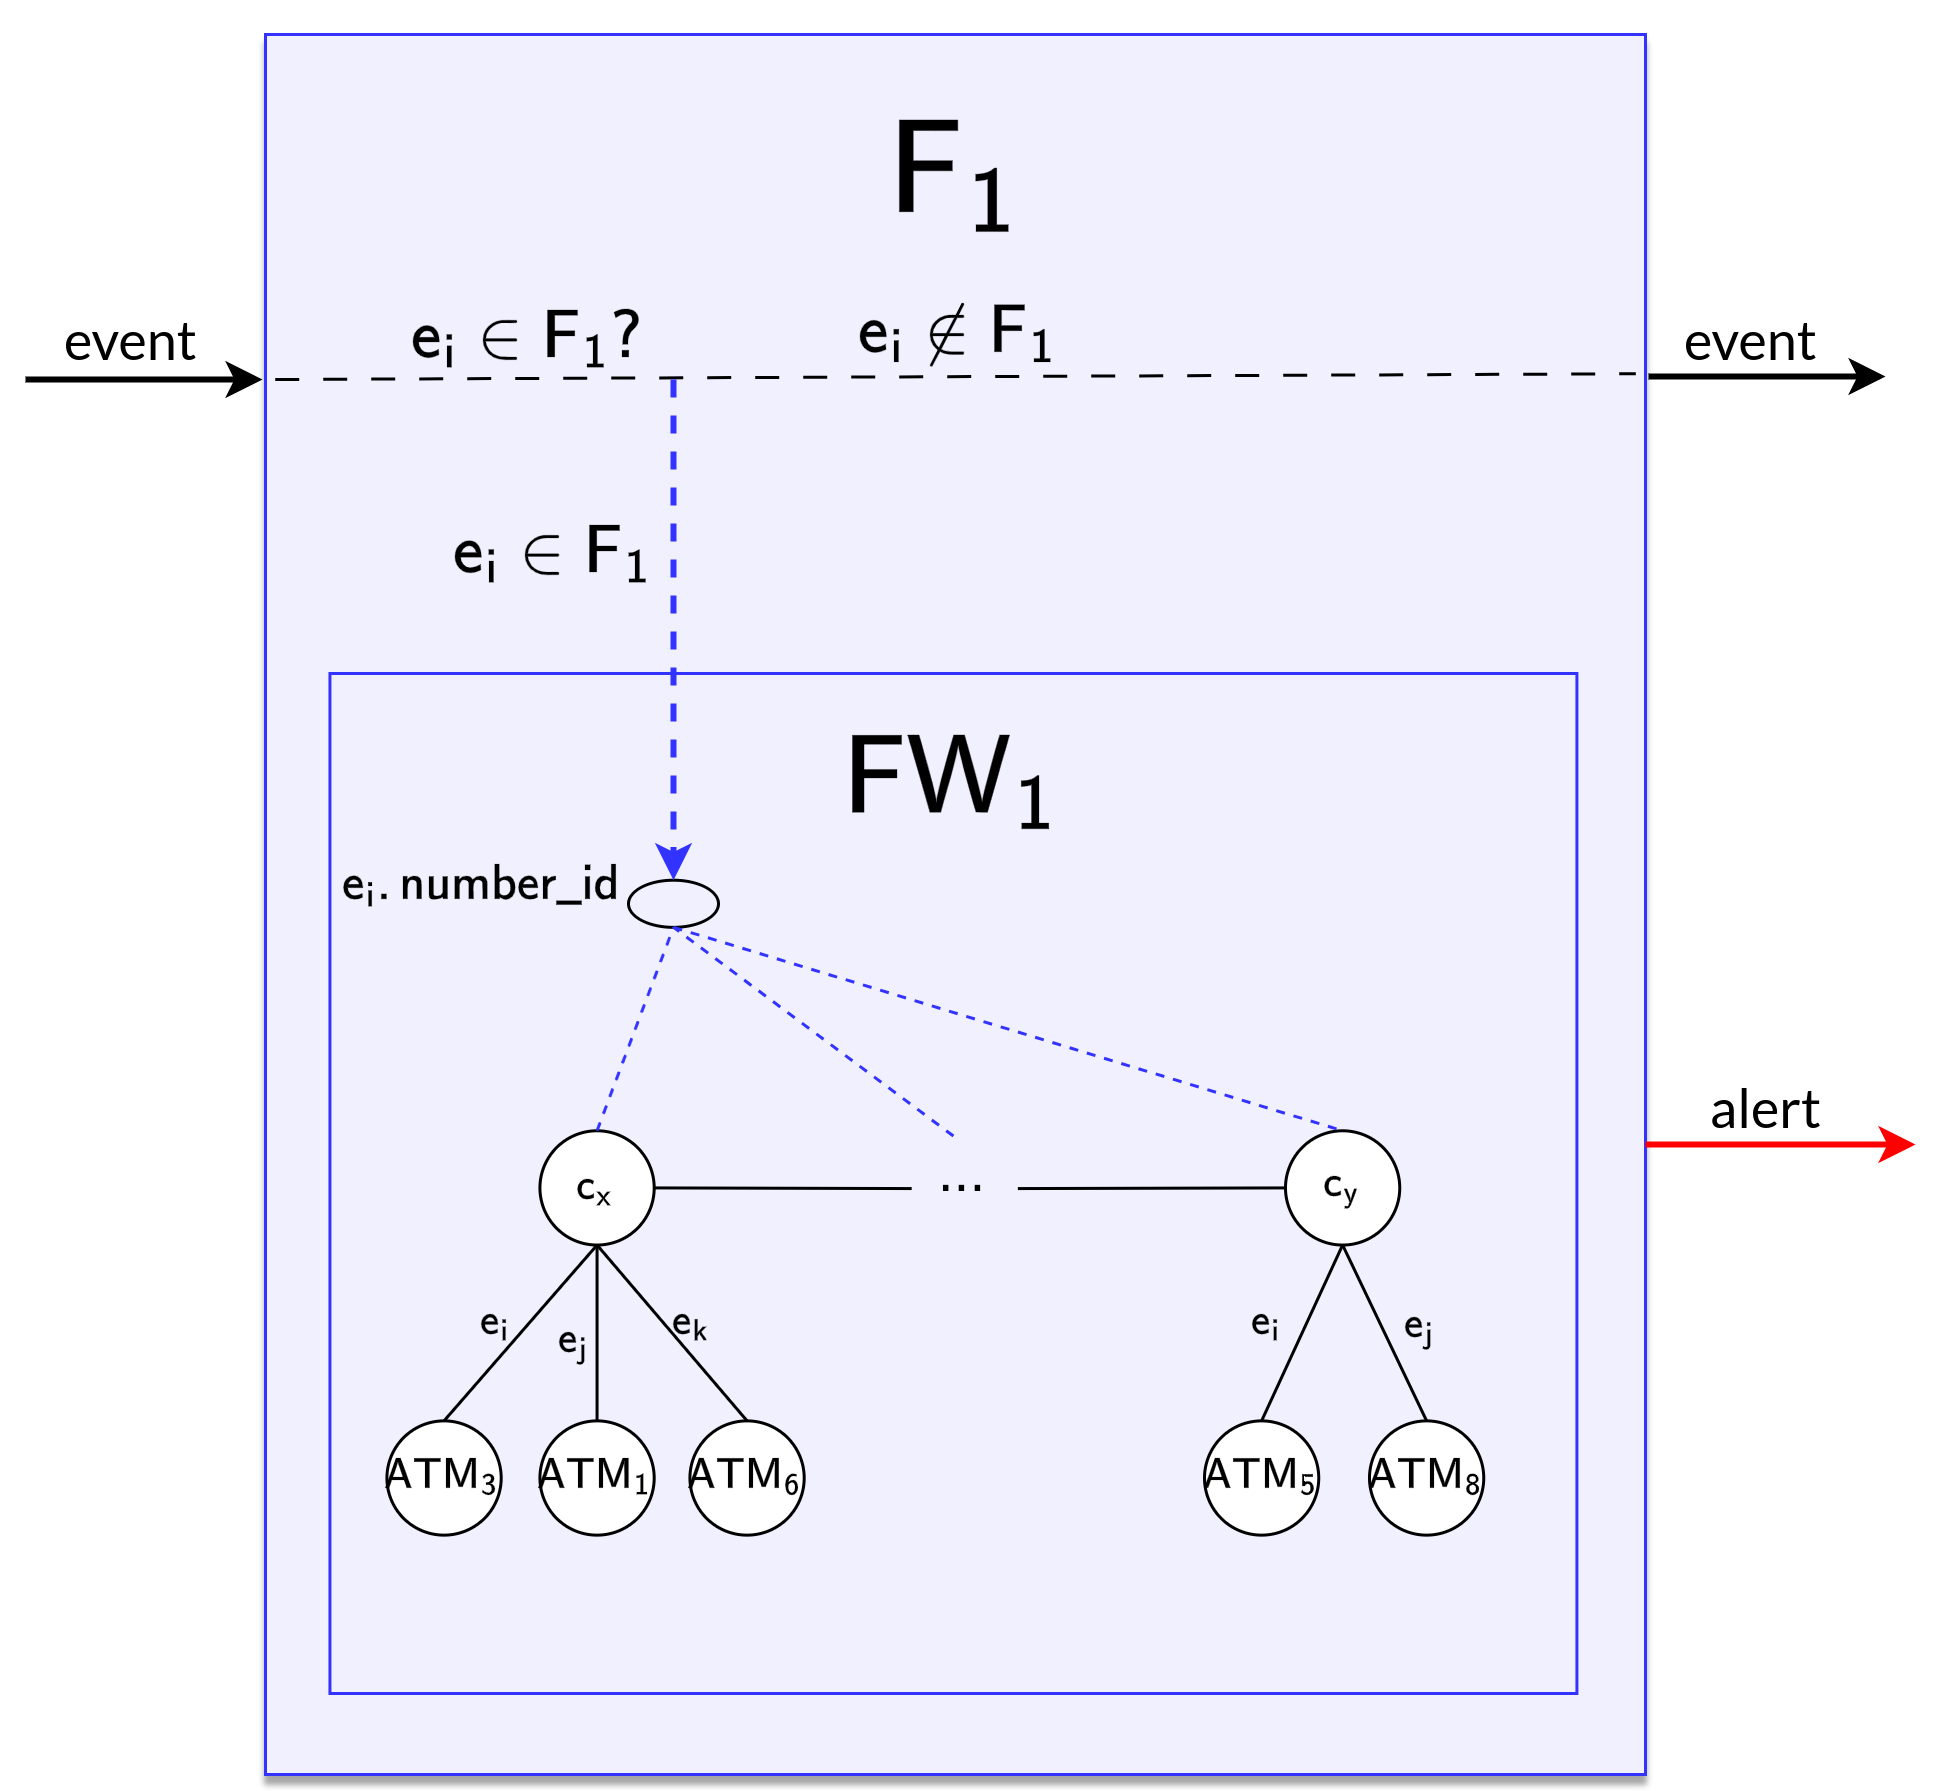
\includegraphics[scale=0.40]{images/3-Engine/filter-worker-subgraphs.png}
        \end{column}
    \end{columns}
\end{frame}

\begin{comment}
\begin{frame}[fragile]{$\mathsf{DP_{ATM}}$ - Filter Stage}
\begin{itemize}
    \item Card cloning fraud pattern algorithmic evaluation
\end{itemize}
    \scalebox{0.9}{ 
    \hspace{-0.7cm}
    \begin{minipage}{1.2\textwidth} 
    \begin{algorithm}[H]
        \caption{\texttt{checkFraud}($\mathsf{S_c, e_{new}}$)}
        \label{alg:check-fraud-impl}
        \begin{algorithmic}[1]
            \Require $\mathsf{S_c}$ is a non-empty subgraph of interaction edges of card $\mathsf{c}$, 
            $\mathsf{e_{new}}$ is the \texttt{Edge} related to the new incoming opening interaction \texttt{EdgeStart} of card $\mathsf{c}$
            \State $\mathsf{e_{last}} \gets S_c[|S_c| - 1]$ \Comment{Retrieve last edge from $\mathsf{S_c}$}
            \If{$\mathsf{e_{last}}.\texttt{Tx\_end}$ is empty}
                \State \texttt{LOG: Warning: A tx ($\mathsf{e_{new}}$) starts before the previous ($\mathsf{e_{last}}$) ends!}
                \Return
            \EndIf
            \If{$\mathsf{e_{last}}.\texttt{ATM\_id} \neq \mathsf{e_{new}}.\texttt{ATM\_id}$}
                \State $\texttt{t\_min} \gets \text{obtainTmin}(\mathsf{e_{last}}, \mathsf{e_{new}})$
                \State $\texttt{t\_diff} \gets \mathsf{e_{new}}.\texttt{Tx\_start} - \mathsf{e_{last}}.\texttt{Tx\_end}$
                \If{$\texttt{t\_diff} < \texttt{t\_min}$}   
                    \State $\text{emitAlert}(\mathsf{e_{last}}, \mathsf{e_{new}})$
                \EndIf
            \EndIf
        \end{algorithmic}
    \end{algorithm}
    \end{minipage}
    }
\end{frame}
\end{comment}

\begin{comment}
\begin{frame}{$\mathsf{DP_{ATM}}$ - Filter Stage}
    \begin{itemize}
         \item \textbf{Filter \emph{worker}}.
         \item Simultaneously (many possible) different continuous query patterns: $FP_1, FP_2, ..., FP_n$.
    \end{itemize}

    \begin{figure}
        \centering
        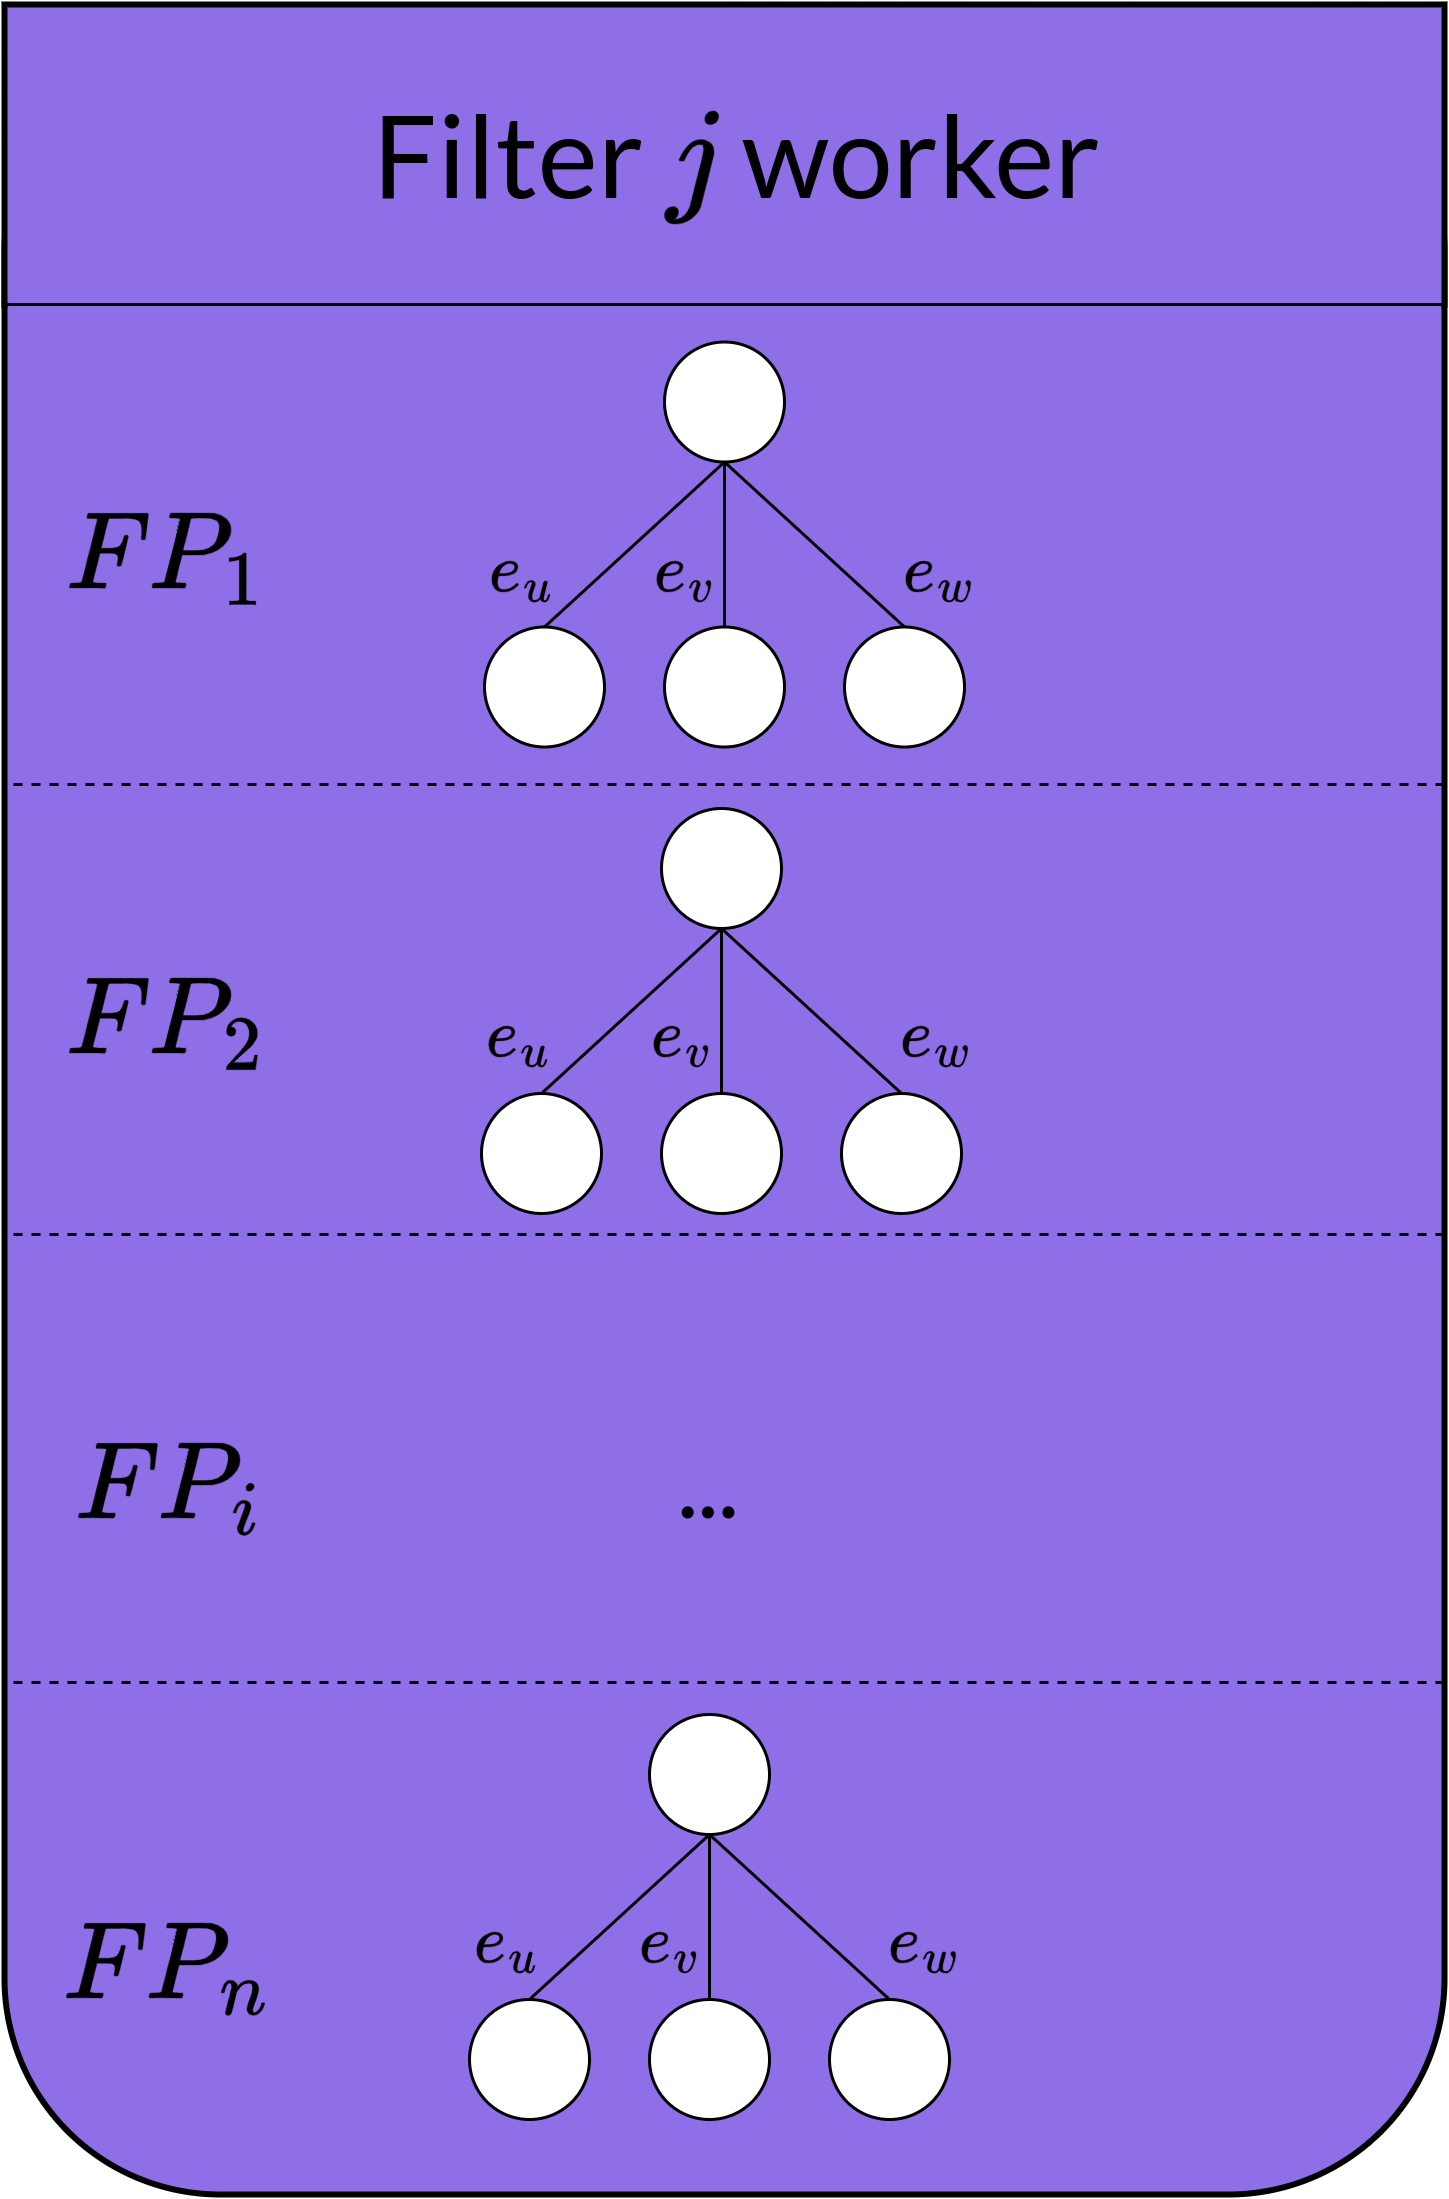
\includegraphics[scale=0.32]{figures/engine-filter-worker-1.png}
   \end{figure}
\end{frame}
\end{comment}

\begin{frame}{Continuous Query Engine - $\mathsf{DP_{ATM}}$: Architecture}
\begin{figure}
    \centering
    \hspace*{-1cm}
    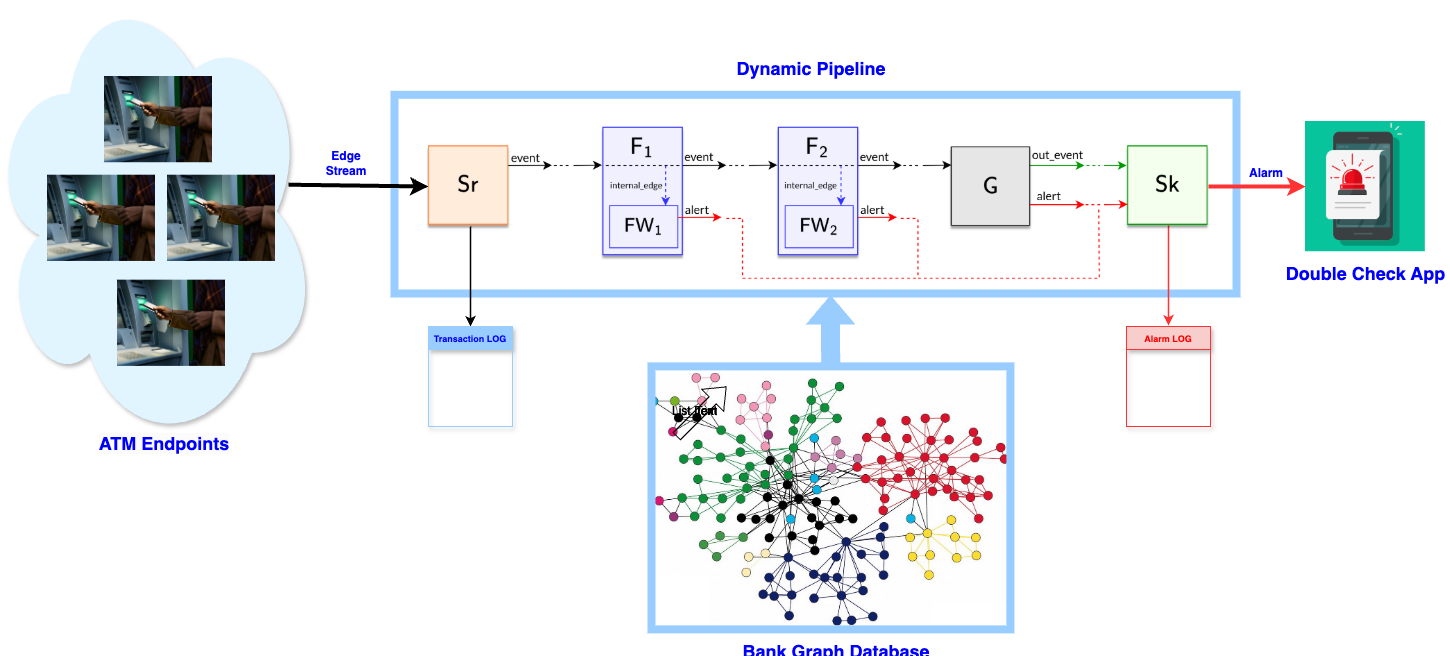
\includegraphics[width=1.18\linewidth]{images/architectureCQE.png}
\end{figure}
\end{frame}
